\documentclass{article}
\usepackage{amssymb}
\usepackage{amsmath}
\usepackage{mathtools}
\usepackage{cancel}
\usepackage{tikz}
\usepackage{hyperref}
\usepackage{circuitikz}
\usepackage{float}
\usepackage{afterpage}
\usepackage{pgfplots}
\pgfplotsset{compat=1.16}
\usepackage{textcomp}
\usepackage{geometry}
\usepackage{tabularx}
\usepackage{esdiff}
\usepackage{siunitx}
\pagenumbering{gobble}


\DeclareMathOperator*{\argmin}{argmin}

\geometry{
    a4paper,
    left=10mm,
    top=10mm,
    right=10mm,
    bottom=15mm
}
\setlength{\extrarowheight}{5pt}

\newcommand{\deriv}[2]{\frac{d{#1}}{d{#2}}}

\begin{document}
\section*{Unilateral Laplace Transform}
$$X(s) = \int_{0^-}^\infty{x(t)e^{-st}dt}$$
\subsection*{Theorems}
\begin{center}
    \begin{tabularx}{\textwidth}{XXX}
        \hline
	$x(t)$ & $X(s)$ & ROC\\
        \hline
	$x(t-t_0)$ & $e^{-st_0}X(s)$ & $R$\\
	$e^{s_0t}x(t)$ & $X(s-s_0)$ & $R + Re(s_0)$\\
	$x(at)$ & $\frac{1}{|a|}X\left( \frac{s}{a} \right)$ & $aR$\\
	$x^*(t)$ & $X(s^*)^*$ & $R$\\
      $(x_1*x_2)(t)$ & $X_1(s)X_2(s)$ & $R_1\bigcap R_2$\\
      $-tx(t)$ & $\diff{X}{s}$ & $R$\\
      $\diff[n]{x}{t}$ & $s^nX(s)-\sum_{i=0}^{n-1}s^{n-i-1}\diff[i]{x}{t}|_{t=0^-}$ & R
    \end{tabularx}
\end{center}
\subsection*{Transforms}
\begin{center}
    \begin{tabularx}{\textwidth}{XXX}
        \hline
        Signal & Transform & ROC\\
        \hline
	$\delta(t-T)$ & $e^{-sT}$ & $\mathbb{C}$\\
	$\frac{t^{n-1}}{(n-1)!}u(t)$ & $\frac{1}{s^n}$ & $Re(s)>0$\\
	$\frac{t^{n-1}}{(n-1)!}e^{-at}u(t)$ & $\frac{1}{(s+a)^n}$ & $Re(s) > a$\\
	$e^{-at}\cos(\omega_0t)u(t)$ & $\frac{s+a}{(s+a)^2+\omega_0^2}$ & $Re(s) > a$\\
	$e^{-at}\sin(\omega_0t)u(t)$ & $\frac{\omega_0}{(s+a)^2+\omega_0}$ & $Re(s) > a$
    \end{tabularx}
\end{center}
\clearpage
\section*{Electro-Mechanical Equivalence}
\subsection*{Equivalent Quantities}
\begin{center}
  \begin{tabularx}{\textwidth}{XXX}
    \hline
    Translational Mechanical System & Rotational Mechanical System & Electrical System \\
    \hline
    Force ($F$) & Torque & Voltage ($V$)\\
    Mass ($M$) & Moment of Inertia ($J$) & Inductance ($L$)\\
    Damping Coefficient ($B$) & Rotational Damping Coefficient ($B$) & Resistance ($R$)\\
    Spring Constant ($K$) & Torsional Spring Constant ($K$) & Reciprocal of Capacitance $\left( \frac{1}{C} \right)$\\
    Displacement ($x$) & Angular Displacement ($\theta$) & Charge ($Q$)\\
    Velocity ($v$) & Angular Velocity ($\omega$) & Current ($I$)
  \end{tabularx}
\end{center}
\subsection*{Equation Equivalence}
\begin{center}
  \begin{tabularx}{\textwidth}{XXX}
    \hline
    Translational Mechanical System & Rotational Mechanical System & Electrical System \\
    \hline
    $Ms^2X(s)$ & $Js^2\Theta(s)$ & $LsI(s)$\\
    $BsX(s)$ & $Bs\Theta(s)$ & $RI(s)$\\
    $KX(s)$ & $K\Theta(s)$ & $\frac{1}{Cs}I(s)$\\
    - & $\frac{T_2(s)}{T_1(s)}=\frac{\Theta_1(s)}{\Theta_2(s)}=\frac{N_2}{N_1}$ & $\frac{N_p}{N_s}=\frac{V_p(s)}{V_s(s)}=\frac{I_s(s)}{I_p(s)}$\\
  \end{tabularx}
\end{center}
\subsection*{Conversion Rules}
\begin{enumerate}
  \item The force at two ends of a damper (or spring) must be equal $\Leftrightarrow$ the voltage across the resistor (or capacitor) must be equal
  \item Parallel in one domain $\implies$ Series in the other domain
  \item $\sum F = 0$ at a massless node $\Leftrightarrow \sum V = 0$ at an electrical node
  \item Rotational impedances are reflected through gear trains by multiplying by $\left( \frac{N^2_{dest}}{N^2_{source}} \right)$
\end{enumerate}
\subsection*{Conversion Procedure}
\subsubsection*{Electrical to Mechanical}
\begin{enumerate}
  \item Label all currents such that only one current flows through inductors
  \item Write loop equations for each loop
  \item Re-write equations using the analogous quantities. Each loop is replaced by a position
  \item Draw mechanical system corresponding to equations
\end{enumerate} 
\subsubsection*{Mechanical to Electrical}
\begin{enumerate}
  \item Write force equations for each position
  \item Re-write equations using analogous quantities. Each equation becomes a loop
  \item Draw loops such that only one current flows through each inductor
\end{enumerate}

\clearpage
\section*{Second-Order System}
\begin{center}
  \[
	H(s) = \frac{\omega_n^2}{s^2+2\zeta\omega_n+\omega_n^2}
  \]
Poles are at $s = -\zeta\omega_n + \omega_n\sqrt{\zeta^2-1}$.
\end{center}
\subsection*{Cases of Interest}
\begin{enumerate}
  \item[] \textbf{$\zeta = 0$}: $s=\pm \omega_nj$. The system is marginally stable.
  \item[] \textbf{$0 < \zeta < 1$}: $s = -\zeta\omega_n\pm j\omega_n\sqrt{1-\zeta^2}$. The system is underdamped.
  \item[] \textbf{$\zeta = 1$}: $s = -\omega_n$. The system is critically damped.
  \item[] \textbf{$\zeta > 1$}: $s = -\zeta\omega_n \pm \omega_n\sqrt{\zeta^2-1}$. The system is overdamped
\end{enumerate}
\subsection*{Underdamped systems}
\begin{enumerate}
  \item[] \textbf{Time to Peak}: $T_p = \frac{\pi}{\omega_n\sqrt{1-\zeta^2}}$
  \item[] \textbf{\% Overshoot}: $e^{\frac{-\zeta\pi}{\sqrt{1-\zeta^2}}}$
  \item[] \textbf{Settling Time}: $T_s = \frac{4}{\zeta\omega_n}$
\end{enumerate}
\textbf{Rule of Thumb:} If two poles are at $s = -a\pm bj$, then if $Re\{c\} \leq 5\cdot Re\{a\}$, the system is approximately second order.
\clearpage
\clearpage
\section*{Bode Diagrams}
\subsection*{First-Order Zeros}
\begin{figure}[!h]
  \centering
  \begin{subfigure}[b]{0.45\textwidth}	
	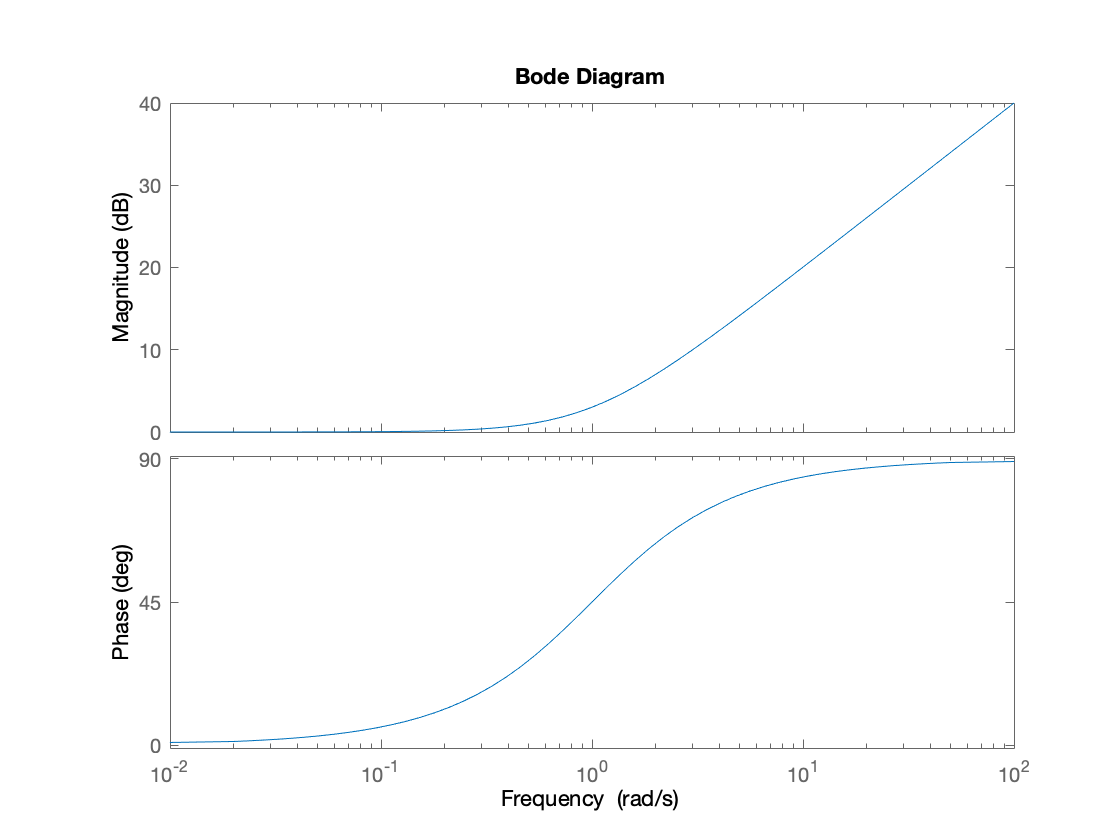
\includegraphics[width=\textwidth]{Images/bode_lhp_zero}
	\caption{LHP Zero}
	\label{fig:bode-lhp-zero}
  \end{subfigure}
  \begin{subfigure}[b]{0.45\textwidth}	
	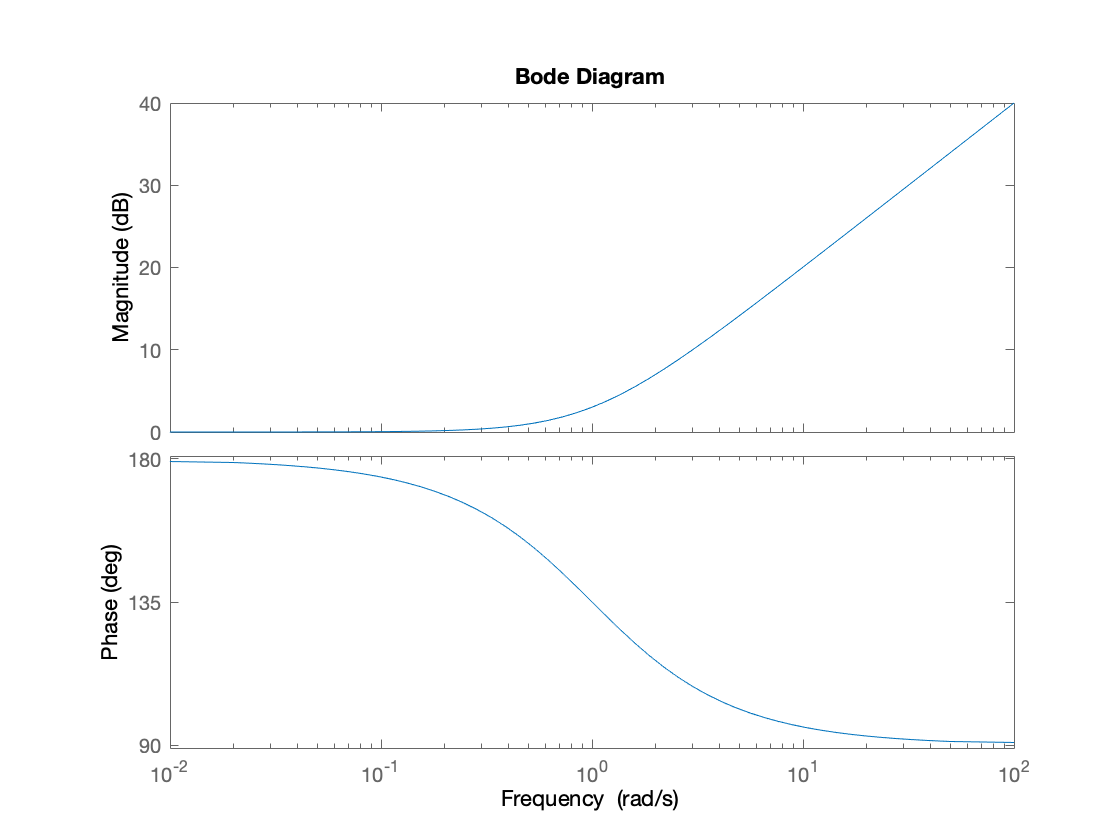
\includegraphics[width=\textwidth]{Images/bode_rhp_zero}
	\caption{RHP Zero}
	\label{fig:bode-rhp-zero}
  \end{subfigure}
\end{figure}
\subsection*{First-Order Poles}
\begin{figure}[!h]
  \centering
  \begin{subfigure}[b]{0.45\textwidth}	
	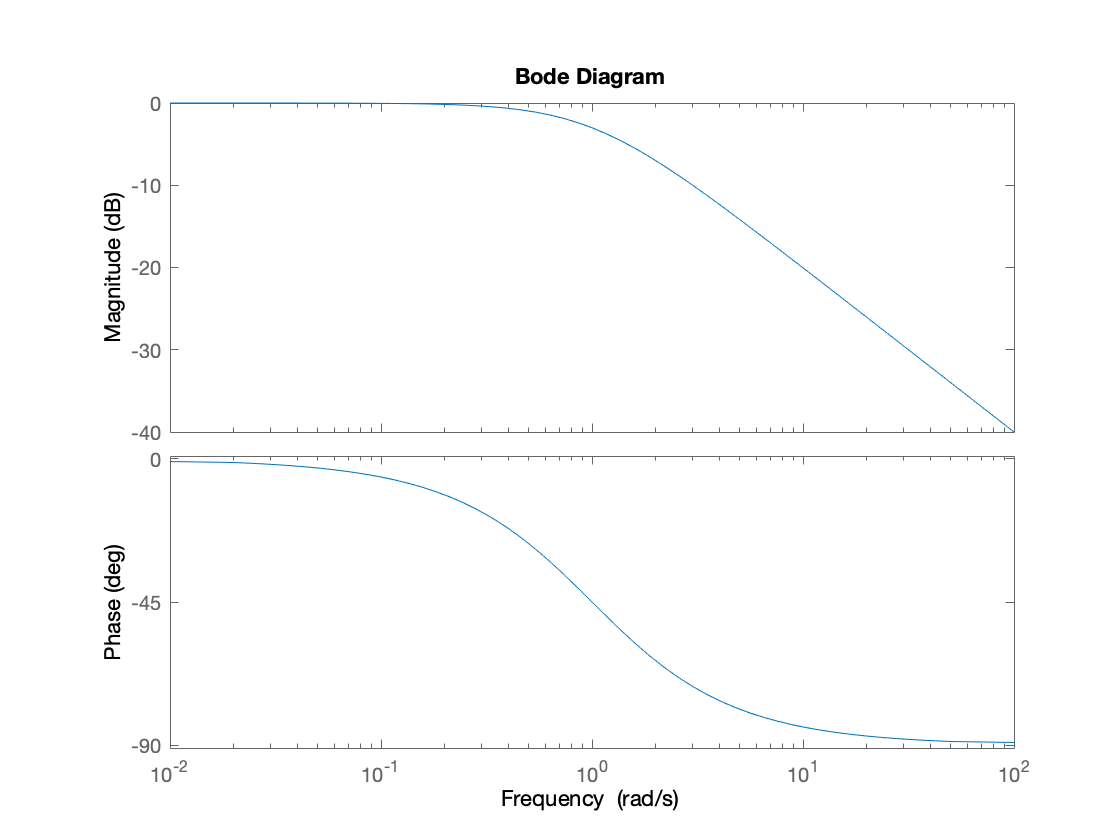
\includegraphics[width=\textwidth]{Images/bode_lhp_pole}
	\caption{LHP pole}
	\label{fig:bode-lhp-pole}
  \end{subfigure}
  \begin{subfigure}[b]{0.45\textwidth}	
	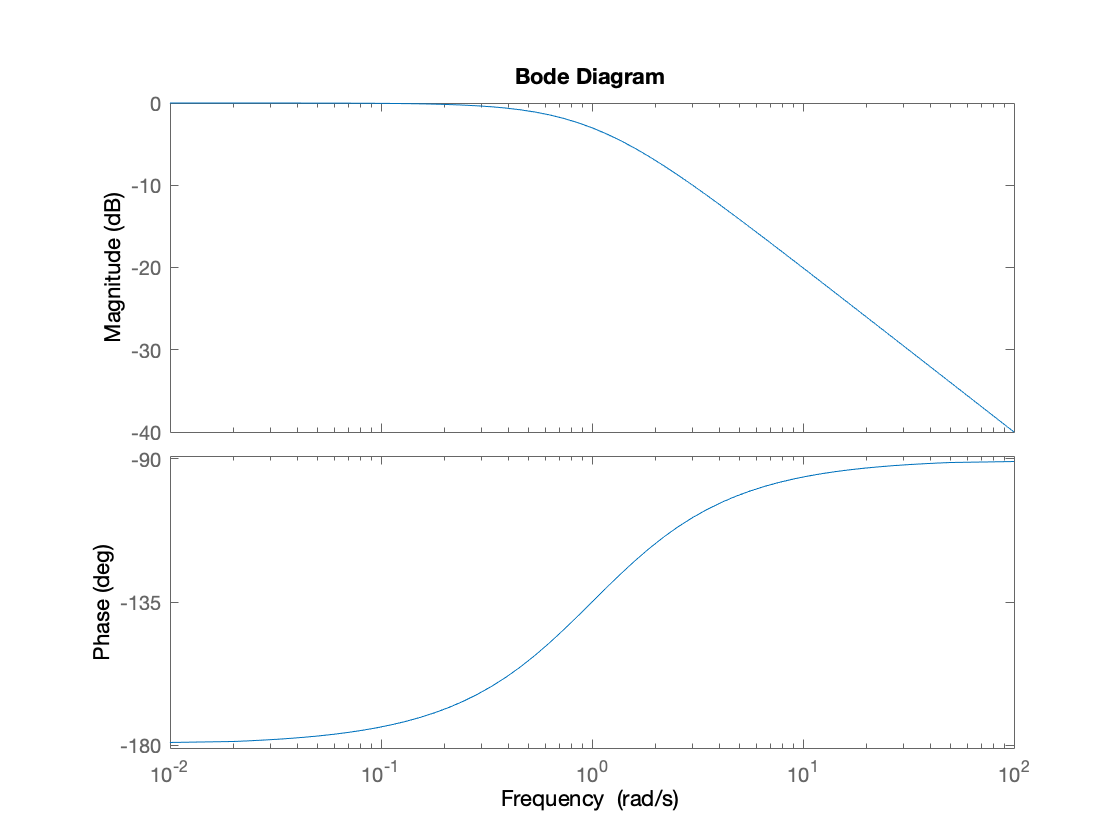
\includegraphics[width=\textwidth]{Images/bode_rhp_pole}
	\caption{RHP Pole}
	\label{fig:bode-rhp-pole}
  \end{subfigure}
\end{figure}
\subsection*{Pole/Zero at $\omega-0$}
\begin{figure}[!h]
  \centering
  \begin{subfigure}[b]{0.45\textwidth}	
	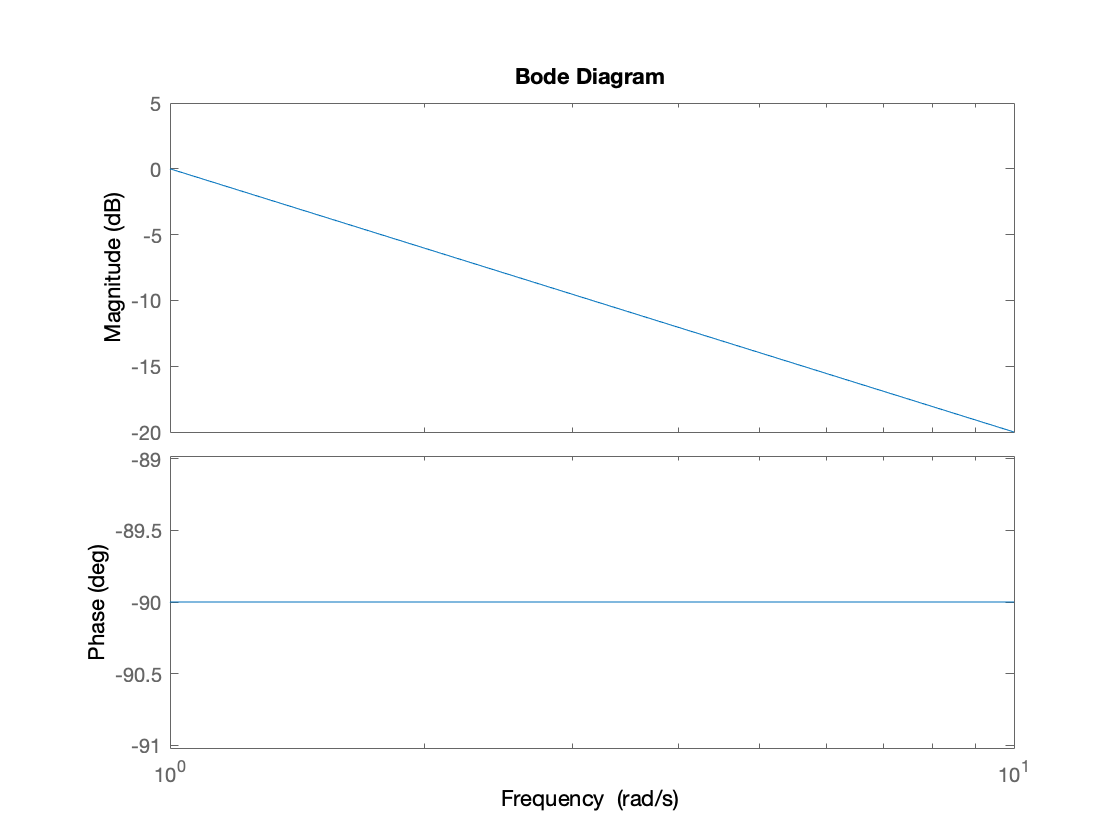
\includegraphics[width=\textwidth]{Images/bode_pole}
	\caption{Pole at zero}
	\label{fig:bode-pole}
  \end{subfigure}
  \begin{subfigure}[b]{0.45\textwidth}	
	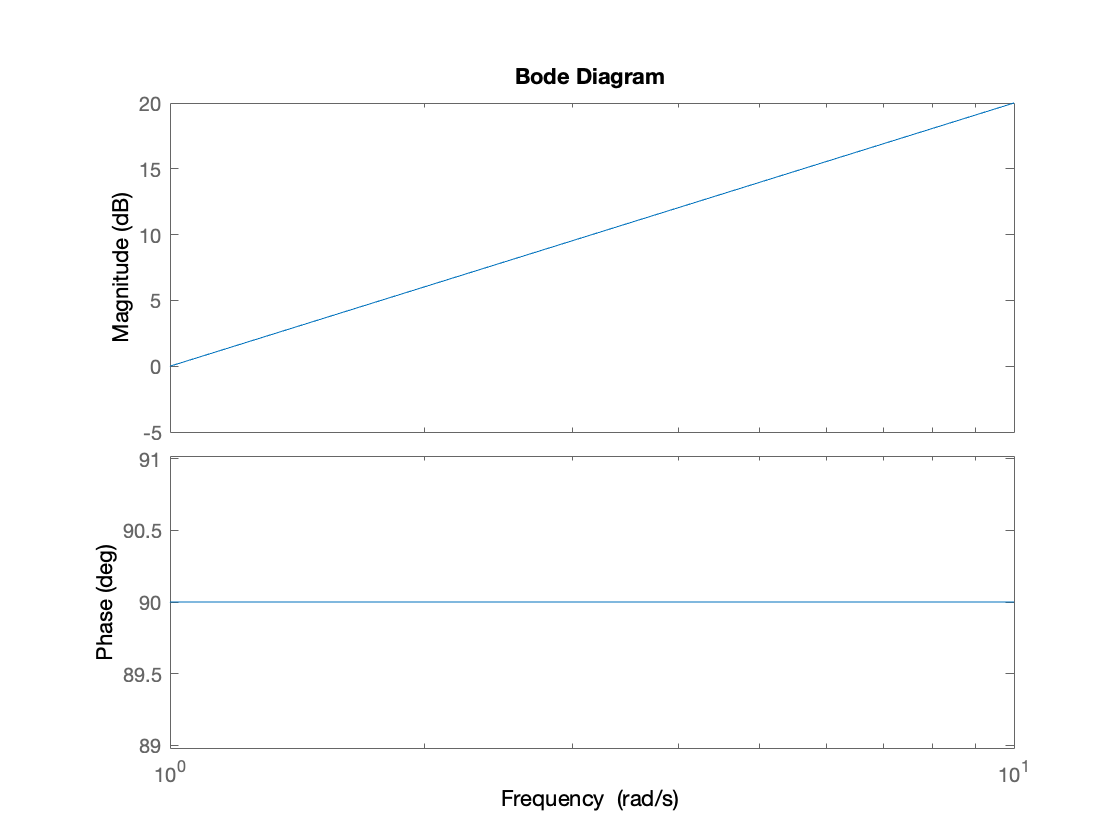
\includegraphics[width=\textwidth]{Images/bode_zero}
	\caption{Zero at zero}
	\label{fig:bode-zero}
  \end{subfigure}
\end{figure}
\subsection*{Second-Order behavior}
\begin{figure}[!h]
  \centering
  \begin{subfigure}[b]{0.45\textwidth}	
	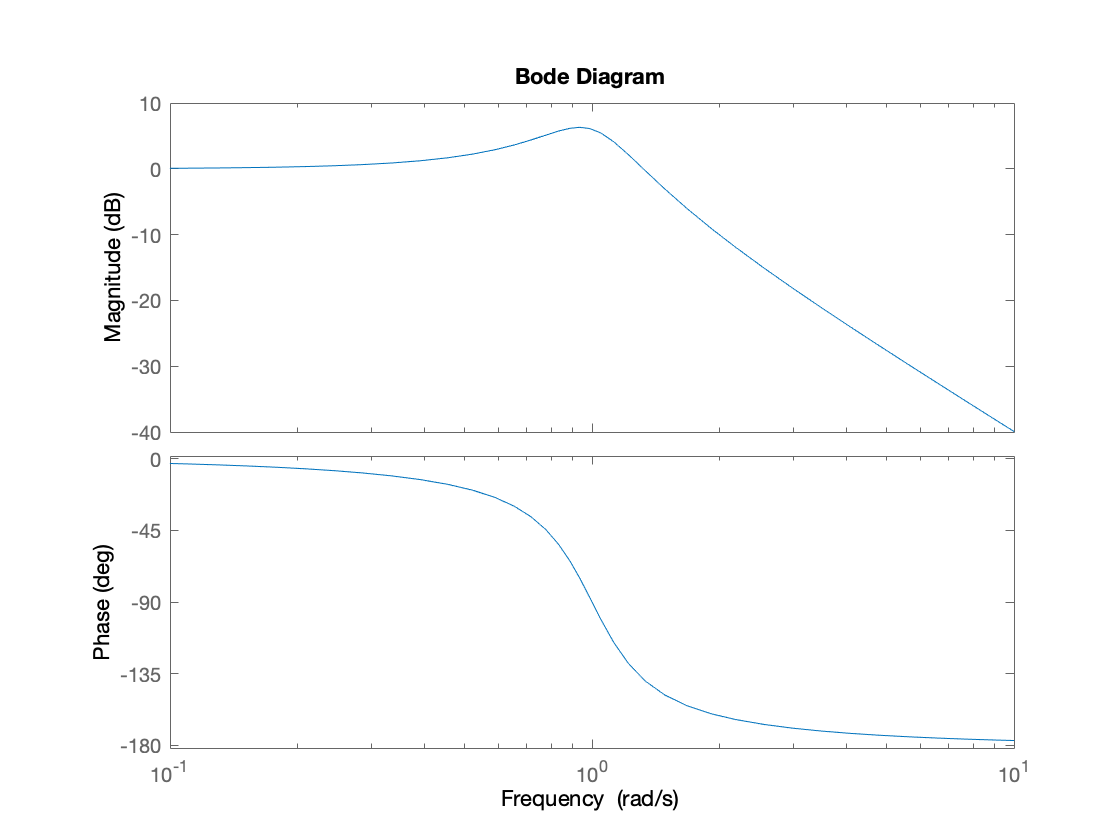
\includegraphics[width=\textwidth]{Images/bode_2nd_order_denom}
	\caption{Second-Order poles}
	\label{fig:bode-2nd-order-pole}
  \end{subfigure}
  \begin{subfigure}[b]{0.45\textwidth}	
	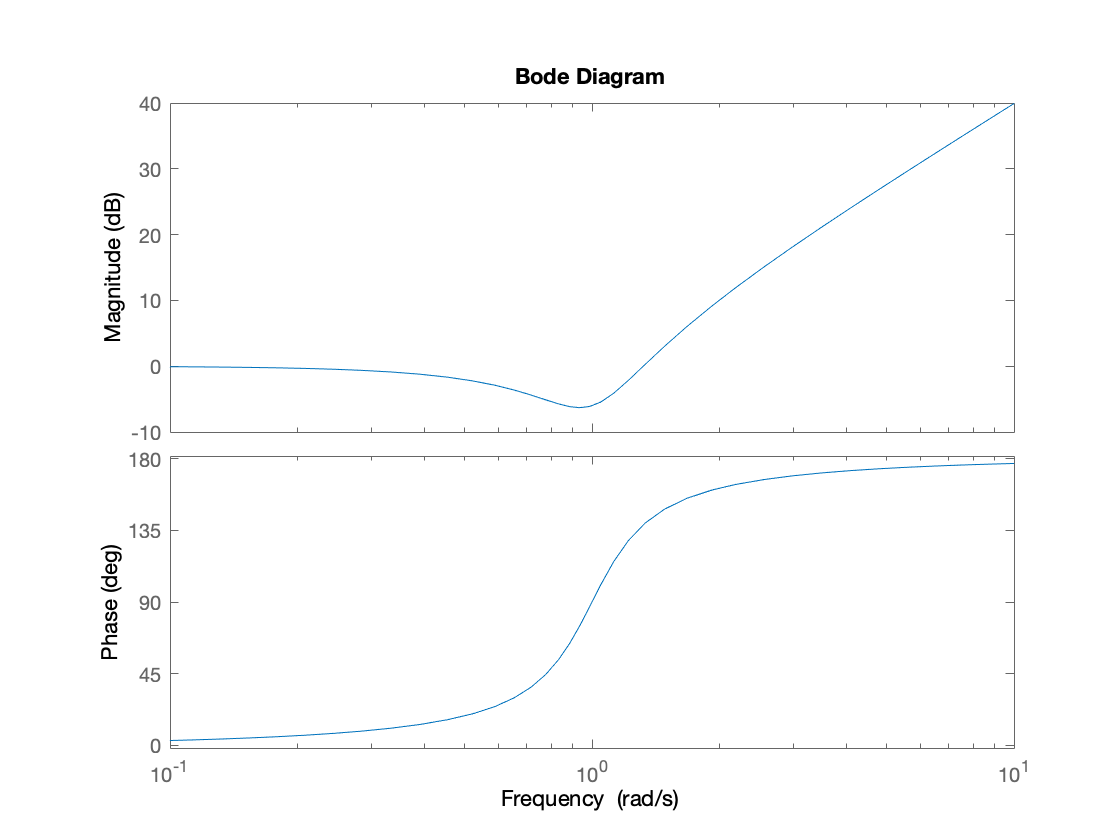
\includegraphics[width=\textwidth]{Images/bode_2nd_order_num}
	\caption{Second-Order zeros}
	\label{fig:bode-2nd-order-zero}
  \end{subfigure}
\end{figure}
\clearpage
\section*{Nyquist Diagrams}
In the standard negative feedback setup with plant $G$ and controller $H$,
\begin{enumerate}
  \item Poles of $1+GH$ are the poles of the open loop system.
  \item Zeros of $1+GH$ are the poles of the closed loop system.
\end{enumerate}
Where $N$ is the number of CCW encirclements of $-1$, $P$ is the number of RHP poles of GH, and $Z$ is number of RHP zeros of $1 + GH$
$$N = P - Z$$
If $Z = 0$, then the system is stable.
\clearpage
\section*{Design by Frequency Response}
\textbf{Gain Margin:} The change in open loop gain that will make the closed loop system unstable.
\[
  \angle G(j\omega_{GM}) = (2k+1)\pi \implies G_m = \frac{1}{G(j\omega_{GM})}
\]
\textbf{Phase Margin:} The change in open loop phase to make the closed loop system unstable.
\[
  |G(j\omega_{PM})| = 1 \implies \phi_{m} = (2k+1)\pi + \angle G(j\omega_{PM})
\]
For a second-order system,
\begin{align*}
  \omega_{PM} &= \omega_n\sqrt{-2\zeta^2+\sqrt{1+4\zeta^4}}\\
  \phi_M &= \tan^{-1}\frac{2\zeta}{\sqrt{-2\zeta^2+\sqrt{1+4\zeta^4}}}
\end{align*}
\subsection*{Lag Controller}
\[
  G_c(s) = \frac{s + \frac{1}{T}}{s + \frac{1}{\alpha T}}, \quad \alpha > 1
\]
\textbf{Purpose:} To reduce static error constant by increasing low frequency gain and to increase the phase margin of the system.
\subsubsection*{Design Procedure}
\begin{enumerate}
  \item Set gain $K$ to the value that satisfies the SSE specification and plot the Bode diagram at that gain.
  \item Find $\omega_{PM}$ such that $\phi_M$ is 5\textdegree  to 12\textdegree  larger than required.
  \item Let the high frequency asymptote be $-20\log K_{PM}$\SI{}{\decibel} at $\omega_{PM}$ where $K_{PM} = |G(j\omega_{PM})|$.
  \item Choose the upper break frequency to be $\frac{\omega_{PM}}{10}$
  \item Set the low frequency asymptote to be \SI{0}{\decibel} and locate the lower break frequency.
  \item Reset the system gain K to compensate for attenuation.
\end{enumerate}
\subsection*{Lead Controller}
\[
  G_c(s) = \frac{1}{\beta}\frac{s+\frac{1}{T}}{s+\frac{1}{\beta T}}, \quad \beta < 1
\]
\textbf{Purpose:} To change the phase margin and decrease percent overshoot and reduce rise/settling time.

The lead controller has a peak phase $\phi_{max}$.
\[
  \omega_{max} = \frac{1}{T\sqrt{\beta}}\quad, \phi_{max} = \sin^{-1}\frac{1-\beta}{1+\beta}, \quad |G_c(j\omega_{max})| = \frac{1}{\sqrt{\beta}}
\]
\subsubsection*{Design Procedure}
\begin{enumerate}
  \item Set gain $K$ of the uncompensated system to a value satisfying SSE requirement.
  \item Plot bode diagram for system with gain $K$ and determine $\phi_M$.
  \item Find $\phi_{M}$ needed to meet requirements and evaluate additional phase contribution from compenstor.
  \item Determine $\beta$.
  \item Determine $|G_c(j\omega_{max})|$.
  \item Determine $\omega_{PM}$ where $|G(j\omega)| = -20\log|G_c(j\omega_{max})|$
  \item Find the break frequencies.
  \item Reset the gain
  \item Simulate and tweak.
\end{enumerate}
\end{document}
